\documentclass[12pt,aspectratio=169]{beamer}
% \hypersetup{pdfpagemode=FullScreen}

\usepackage{upgreek}
\usefonttheme{professionalfonts}

\renewcommand*{\thefootnote}{\fnsymbol{footnote}}

\makeatletter
\def\onlyfootnote{\gdef\@thefnmark{}\@footnotetext}
\makeatother

\mode<presentation>
\useoutertheme[subsection=false]{miniframes}

\AtBeginSection[]{
  \begin{frame}
  \centering
  \begin{beamercolorbox}[sep=8pt,center,shadow=true,rounded=true]{title}
    \usebeamerfont{title}\insertsectionhead\par%
  \end{beamercolorbox}
  \end{frame}
}

\title{FreeTensor: A Free-Form DSL with Holistic Optimizations for Irregular Tensor Programs}
\author{Shizhi Tang\inst{1}\and Jidong Zhai\inst{1}\and Haojie Wang\inst{1}\and Lin Jiang\inst{1}\and Liyan Zheng\inst{1}\and Zhenhao Yuan\inst{1}\and Chen Zhang\inst{1}}
\institute{\inst{1}Tsinghua University}
\date{Presenter: Shiwei Zhang}

\begin{document}
    \beamertemplatenavigationsymbolsempty

    \makeatletter
    \def\beamer@andinst{\\[.1em]}
    \makeatother

    \begin{frame}
        \titlepage
    \end{frame}



    \section*{Content}

    \begin{frame}
        \frametitle{Content}

        \begin{itemize}
            \setlength{\itemsep}{.8em}
            \item Introduction
            \item Background and Motivation
            \item Free-Form DSL
            \item Code Generation
            \item Evaluation
            \item Conclusion
        \end{itemize}
    \end{frame}



    \section{Introduction}

    \begin{frame}
        \frametitle{Irregular Tensor Programs}

        \begin{columns}
            \begin{column}{0.5\textwidth}
                Current tensor programming frameworks (Tensorflow, PyTorch, etc.) work on whole-tensor level.

                \vskip 1em
                Irregular tensor programs usually include \textbf{fine-grained operations} that only use a part
                of a tensor and \textbf{combination of multiple operations} that should be fused.
            \end{column}
            \begin{column}{0.5\textwidth}
                \vskip -1em
                \includegraphics[page=2,trim=1.95cm 18.2cm 10.5cm 2.2cm,clip,scale=.8]{paper.pdf}
            \end{column}
        \end{columns}
    \end{frame}

    \begin{frame}
        \frametitle{Free-Form Tensor Programs}

        \begin{columns}
            \begin{column}{0.5\textwidth}
                \includegraphics[page=5,trim=1.9cm 8.5cm 10.5cm 12cm,clip,scale=.8]{paper.pdf}
            \end{column}
            \begin{column}{0.5\textwidth}
                \vskip -1em
                \includegraphics[page=2,trim=1.95cm 18.2cm 10.5cm 2.2cm,clip,scale=.8]{paper.pdf}
            \end{column}
        \end{columns}
    \end{frame}

    \begin{frame}
        \frametitle{Contributions}

        \begin{itemize}
            \setlength{\itemsep}{.8em}
            \item FreeTensor DSL to express free-form tensor programs.
            \item Holistic compilation optimizations including partial evaluation, denpendence-aware transformation, and automatic code generation for different architectures.
            \item Fine-grained automatic differentiation (AD) with selective tensor materialization (gradient checkpointing).
            \item Evaluation shows that compared to PyTorch, JAX, TVM, Julia, and DGL, FreeTensor achieves up to 5.10x speedup (2.08x on average) without AD and up to 127.74x speed up (36.26x on average) with AD.
        \end{itemize}
    \end{frame}



    \section{Background and Motivation}

    \begin{frame}
        \frametitle{Current State}

        \begin{itemize}
            \setlength{\itemsep}{.8em}
            \item \textbf{Tensorflow} and \textbf{PyTorch} use optimized libraries (cuDNN, cuBLAS, Intel MKL) for computation. New kernels have to be developed for new operations used in new models.
            \item \textbf{TVM} is proposed to reduce manual efforts in writing new kernels. However, it does not support irregular tensor programs.
            \item \textbf{Julia} is a general purpose programming language that is capable of expressing irregular tensor programs, but it fails to generate high-performance code due to lacking domain knowledge.
        \end{itemize}
    \end{frame}

    \begin{frame}
        \frametitle{Motivating Example}


        \begin{columns}
            \begin{column}{0.6\textwidth}
                The same operation expressed with free-form tensor program does not include redundant operators
                (indexing, reshape, cat, etc.) and does not use extra memory.

                \vskip 1em
                \centering
                \includegraphics[page=4,trim=2.2cm 9.8cm 10.5cm 12cm,clip,scale=.7]{paper.pdf}
            \end{column}
            \begin{column}{0.4\textwidth}
                \centering
                \vskip -2.5em
                \includegraphics[page=3,trim=11cm 11cm 2cm 3cm,clip,scale=.62]{paper.pdf}
            \end{column}
        \end{columns}
    \end{frame}

    \begin{frame}
        \frametitle{Challenges}

        \begin{itemize}
            \setlength{\itemsep}{.8em}
            \item \textbf{Optimization with dependence}. Fine-grained control flow introduced by FreeTensor often contain data dependence that hinder potential code transformation.
            \item \textbf{Efficient automatic differentiation on complex control flows}. Loops often create a large number of intermediate tensors with AD. FreeTensor incorperates selective tensor materialization to mitigate this problem.
        \end{itemize}
    \end{frame}



    \section{Free-Form DSL}

    \begin{frame}
        \frametitle{Tensor definition and indexing}

        \centering
        \includegraphics[page=4,trim=10.5cm 6.5cm 2cm 17cm,clip]{paper.pdf}
    \end{frame}

    \begin{frame}
        \frametitle{Granularity-Oblivious Tensor Operations}

        \begin{columns}
            \begin{column}{0.5\textwidth}
                With \textbf{integer ranged for-loops}, \textbf{branches}, and \textbf{always-inlined function calls},
                FreeTensor supports tensor operations in any granularity.
            \end{column}
            \begin{column}{0.5\textwidth}
                \includegraphics[page=5,trim=1.9cm 8.5cm 10.5cm 12cm,clip,scale=.9]{paper.pdf}
            \end{column}
        \end{columns}
    \end{frame}

    \begin{frame}
        \frametitle{Dimension-Free Programming}

        \begin{columns}
            \begin{column}{0.48\textwidth}
                Metadata of tensors are tracked and accessible within FreeTensor. This allows the user to write functions
                that work on tensors with different numbers of dimensions.
            \end{column}
            \begin{column}{0.52\textwidth}
                \includegraphics[page=5,trim=11.2cm 6cm 1.9cm 14cm,clip,scale=.88]{paper.pdf}
            \end{column}
        \end{columns}
    \end{frame}



    \section{Code Generation}

    \begin{frame}
        \frametitle{Stack-Scoped Abstract Syntax Tree (AST)}

        \begin{columns}
            \begin{column}{0.5\textwidth}
                Stack-scoped: variables are restricted in subtrees.
                \vskip 1em
                \includegraphics[page=6,trim=2cm 8.5cm 10.5cm 14.5cm,clip,scale=.9]{paper.pdf}
            \end{column}
            \begin{column}{0.5\textwidth}
                \includegraphics[page=5,trim=1.9cm 8.5cm 11cm 12cm,clip,scale=.9]{paper.pdf}
            \end{column}
        \end{columns}
    \end{frame}

    \begin{frame}
        \frametitle{Partial Evaluation}

        \begin{columns}
            \begin{column}{0.5\textwidth}
                FreeTensor first evaluates the program using only the metadata (dimensions and shapes of tensors) to inline the recursive function calls.
                \vspace{4em}
            \end{column}
            \begin{column}{0.5\textwidth}
                \vskip -1.8em
                \includegraphics[page=7,trim=2cm 4.4cm 11.4cm 13cm,clip,scale=.85]{paper.pdf}
            \end{column}
        \end{columns}
    \end{frame}

    \begin{frame}
        \frametitle{Dependence-Aware Transformation}

        \begin{columns}
            \begin{column}{0.5\textwidth}
                The next step is to perform a series of transformations, each turns the AST into an equivalent but more
                efficient AST.
                \vskip 1em
                However, some of the transformations are not applicable with the presence of data dependence. FreeTensor
                uses a polyhedral analysis tool called isl to detect these cases.
            \end{column}
            \begin{column}{0.5\textwidth}
                \vskip -1.8em
                \includegraphics[page=6,trim=10.5cm 17.4cm 2cm 2.2cm,clip,scale=.85]{paper.pdf}
            \end{column}
        \end{columns}
    \end{frame}

    \begin{frame}
        \frametitle{AST Transformation}

        \centering
        \includegraphics[page=7,trim=2cm 10cm 2cm 3cm,clip,scale=.75]{paper.pdf}
    \end{frame}

    \begin{frame}
        \frametitle{AST Transformation Strategy}

        FreeTensor allows users to choose any transformation to apply on any statement. On the other hand, it also provides
        a heuristic that greedly applies 6 passes of transformations.

        \vskip .5em
        \begin{itemize}
            \item \texttt{auto\_fuse}: fuse loops to increase locality.
            \item \texttt{auto\_vectorize}: implement loops with vector instructions.
            \item \texttt{auto\_parallel}: bind loops to threads.
            \item \texttt{auto\_mem\_type}: try to put tensors near to processors (registers $>$ scratch-pad memory $>$ main memory).
            \item \texttt{auto\_use\_lib}: replace certain operations with external libraries.
            \item \texttt{auto\_unroll}: unroll short loops to allow downstream optimizations.
        \end{itemize}
    \end{frame}

    \begin{frame}
        \frametitle{Native Code Generation}

        FreeTensor applies further optimizations on the AST after transformations, including simplification on
        mathematical expressions, merging or removing redundant memory access, and removing redundant branches.
        FreeTensor also performs some backend-specific post-processing including inserting thread synchronizing
        statements, generating parallel reduction statements, and computing offsets of tensors in scratch-pad memory.

        \vskip 1em After that, FreeTensor generates OpenMP or CUDA code from the AST and invoke dedicated backend
        compilers like gcc or nvcc for further lower-level optimizations, and native code generations.
    \end{frame}

    \begin{frame}
        \frametitle{Automatic differentiation}

        \begin{columns}
            \begin{column}{0.55\textwidth}
                Each write-after-read (WAR) dependency on the tensor corresponds to a version that need to be saved for
                backward pass. FreeTensor decides whether a tensor should be materialized at compile time.
            \end{column}
            \begin{column}{0.45\textwidth}
                \centering
                \vskip -2em
                \includegraphics[page=10,trim=11.5cm 9cm 2cm 9cm,clip,scale=.8]{paper.pdf}
            \end{column}
        \end{columns}
    \end{frame}



    \section{Experiments}

    \begin{frame}
        \frametitle{Experimental Setup}

        \textbf{Hardware}: A server with dual 12-core CPU and a V100 (32G).
        \vskip 1em
        \textbf{Baselines}: PyTorch 1.8.1, Jax 0.2.19, TVM (Nov 4, 2021), Julia 1.6.3, and DGL 0.7.1.
        \vskip 1em
        \textbf{Workloads}:\\
        ~~- SubdivNet: a CNN for predicting properties of 3D objects.\\
        ~~- Longformer: a Transformer that only considers nearby tokens.\\
        ~~- SoftRas: a differentiable 3D rendering software.\\
        ~~- GAT: a GNN that uses attention for aggregation.
    \end{frame}

    \begin{frame}
        \frametitle{End-to-End Performance without AD}

        \includegraphics[page=12,trim=2.2cm 19.5cm 2.2cm 2.2cm,clip,scale=0.8]{paper.pdf}
    \end{frame}

    \begin{frame}
        \frametitle{End-to-End Performance with AD}

        \includegraphics[page=12,trim=2.2cm 12.8cm 2.2cm 9.2cm,clip,scale=0.8]{paper.pdf}
    \end{frame}

    \begin{frame}
        \frametitle{Analysis of the Speedup}

        By avoiding redundant tensors and using fewer operators, FreeTensor significantly reduces the numbers of kernel
        invocations, memory and cache access, and FLOPs.

        \vskip 1em
        \includegraphics[page=13,trim=2.2cm 21.5cm 2.2cm 2.2cm,clip,scale=0.8]{paper.pdf}
    \end{frame}

    \begin{frame}
        \frametitle{Optimization for AD}

        For any tensors that FreeTensor decided to recompute it rather than to materialize it, there is a pure
        performance gain in a forward pass, since we no longer need to allocate memory and write to the memory for the
        materialization. As for a backward pass, there will also be a performance gain if the recomputing overhead is
        less than the reusing overhead.

        \vskip 1em
        \includegraphics[page=13,trim=2.2cm 17cm 2.2cm 8cm,clip,scale=0.8]{paper.pdf}
        \onlyfootnote{*FT(\texttt{+}) and FT(\texttt{-}) denote using and not using selective tensor materialization}
    \end{frame}

    \begin{frame}
        \frametitle{Compiling Time}

        \centering
        \includegraphics[page=14,trim=2.2cm 13.5cm 11cm 10cm,clip,scale=1]{paper.pdf}
        \onlyfootnote{*ICE means internal compiler error}
    \end{frame}



    \section{Summary}

    \begin{frame}
        \frametitle{Strength}

        \begin{itemize}
            \setlength{\itemsep}{.8em}
            \item New approach (polyhedral analysis) to solve new problem (irregular tensor programs).
            \item Diverse baselines and benchmark models, with deep analysis for the speedup.
            \item A lot of concret code examples.
        \end{itemize}
    \end{frame}

    \begin{frame}
        \frametitle{Limitation}

        \begin{itemize}
            \setlength{\itemsep}{.8em}
            \item The optimization strategy is greedy and not cost-based. We don't know if they hand-tuned the heuristics for the benchmark models.
            \item The benchmark models are all related to convolution operations, while they do not implement them with the convolution operation provided by cuDNN.
            \item They duplicates some optimizations that would be performed by the backend compiler (gcc and nvcc). Further, the backend compiler may override some decisions made by FreeTensor, like loop fusion, reordering, and unrolling.
            \item Only supports fully static graphs with the shapes of all tensors known at compile time.
        \end{itemize}
    \end{frame}

    \begin{frame}
        \frametitle{Takeaways}

        \begin{itemize}
            \setlength{\itemsep}{.8em}
            \item New models bring new challenges and opportunities to machine learning systems.
            \item We can find inspiration from other areas, like non-ML distributed systems and non-ML compiler techniques.
        \end{itemize}
    \end{frame}

    \appendix

    \begin{frame}
        \vskip 1em

        \centering \huge
        Thank you!
    \end{frame}
\end{document}
